\documentclass[12pt,letterpaper]{article}
\title{OpenGL Notes}
\author{G H Lathrom}

\usepackage{mystyle}
\usepackage{wasysym}
\usepackage{tensor}
\usepackage[all,cmtip]{xy}
%\usepackage{txfonts}
%\usepackage{stmaryrd}
\usepackage[dvips]{graphicx}
\usepackage[margin=1in,includehead]{geometry}
\usepackage{hyperref}

\newcommand{\lspan}{\operatorname{span}}
\newcommand{\Ob}{\operatorname{Ob}}
\newcommand{\id}{\operatorname{id}}
\newcommand{\diag}{\operatorname{diag}}
\newcommand{\SO}{\operatorname{SO}}
\newcommand{\Oth}{\operatorname{O}}
\newcommand{\supp}{\operatorname{supp}}
\newcommand{\invlim}{\varprojlim}

\renewcommand{\theenumi}{\alph{enumi}}
\renewcommand{\hat}{\widehat}

\begin{document}
\maketitle

%%%%%%%%%%%%%%%%%%%%%%%%%%%%%%%%%
%%% Header Style
%%%%%%%%%%%%%%%%%%%%%%%%%%%%%%%%%

\pagestyle{fancy}
\fancyhf{}
\lhead{\slshape OpenGL Notes}
\chead{}
\rhead{\slshape G H Lathrom}
\fancyfoot[C]{\thepage}
%\renewcommand{\chaptermark}[1]{\markboth{\chaptername \ 
%\thechapter. \ #1}{}} 
\renewcommand{\headrulewidth}{.5pt}
%%%%%%%%%%%%%%%%%%%%%%%%%%%%%%%%%
%\tableofcontents

For opening a simple window the necessary structure is basically the following:
\begin{enumerate}
    \item Initialize the Graphics Library Framework (glfw).
    \item Provide Hints for Configuration. (optional)
    \item Create the window.
    \item Point current context to new window.
    \item Initialize GLEW.
    \item Create the Window Loop:
        \begin{enumerate}
            \item Poll Events.
            \item Perform Operations on Window.
            \item Swap buffers back to front.
        \end{enumerate}
    \item Terminate the window.
\end{enumerate}


\cite{babyrudin}

The blue regions represent areas in which we may inject our own shaders.

\begin{figure}[htpb]
    \begin{center}
        \begin{minipage}[t]{.8\textwidth}
            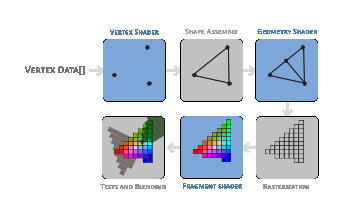
\includegraphics[width=\textwidth]{images/pipeline.eps}
        \end{minipage}
    \end{center}
    \caption{OpenGL Graphics Pipeline}
    \label{fig:pipeline}
\end{figure}


\bibliographystyle{amsalpha}
\bibliography{thebibliography}

\end{document}
